In diesem Abschnitt werden alle Netzwerke hinsichtlich ihrer Trainingsdauer untersucht. Die Trainingszeit wird in jedem Plot angegeben und ist im Wesentlichen abhängig von der Anzahl der verwendeten Trainingsdaten sowie der maximal erlaubten Epochenanzahl. Daher werden für die 
Klassifikations- und Regressionsnetzwerke jeweils gleiche Mengen an Trainingsdaten und identische Gesamtepochenzahlen verwendet.

Beim Einsatz von TF kommen stets der kleinste Target-Datensatz sowie der größte Source-Datensatz zum Einsatz. Ohne TF wird 
ausschließlich der kleinste Target-Datensatz verwendet. Jedes Klassifikationsnetzwerk wird über insgesamt 40 Epochen trainiert, wobei bei 
Anwendung von TF nach 20 Epochen gewechselt wird. Regressionsnetzwerke werden über 80 Epochen trainiert, mit einem TF-Wechsel nach 30 Epochen.

Die entsprechenden Graphen werden an dieser Stelle nicht dargestellt, da deren Anzahl zu groß ist und vergleichbare Darstellungen bereits an 
anderen Stellen verfügbar sind. Für die Einsichtnahme und Überprüfung dieser Ergebnisse verweisen wir auf das zugehörige GitHub-Repository 
unter \url{https://github.com/Lirras/BA_EvalTF_DDCN/tree/main/Plots/ba_plots/timing}. 

Es wird keine Early-Stopping-Metrik verwendet. Alle Klassifikationsnetzwerke erhalten identische Eingabedaten, ebenso wie alle 
Regressionsnetzwerke, um eine bessere Vergleichbarkeit innerhalb der jeweiligen Gruppe zu gewährleisten. Die verschiedenen Netzversionen – 
Cascade TF, Cascade und Complete – besitzen dabei dieselben Layer in gleicher Anzahl.

Im Folgenden wird eine Tabelle präsentiert, die die Trainingszeiten aller Netzwerke in einer vergleichbaren Form zusammenfasst:

\begin{table}[h!]
    \begin{center} 
        \begin{tabular}{l|l|l|l}
            \textbf{Netzwerk} & \textbf{Cascade TF} & \textbf{Cascade} & \textbf{Complete} \\
            \hline
            ConvMaxPool & 78 & 25 & 20 \\
            1DConv & 207 & 34 & 30 \\
            ClassOneDense & 79 & 28 & 13 \\
            RegressionTwo & 11 & 12 & 17 \\
            OneLayer & 16 & 18 & 11
        \end{tabular}
        \caption{
            \small{Dies stellt den Vergleich der Trainingsdauer zwischen den jeweiligen Netzwerken und deren Varianten dar. Die Zeitangaben erfolgen in Sekunden.}}
        \label{tab:time}
    \end{center}
\end{table}

In Tabelle \ref{tab:time} sind die Trainingszeiten der unterschiedlichen Netzwerkvarianten zusammengefasst. Die Spalte "Cascade TF" umfasst 
Kaskadennetzwerke mit TF. Die Spalte "Cascade" enthält Kaskadennetzwerke, die ausschließlich auf dem Target-Datensatz 
trainiert wurden. Die Spalte "Complete" schließlich zeigt die Trainingszeiten von Netzwerken, die weder TF verwenden noch kaskadiert sind, deren 
Layer vor dem Training festgelegt wurden und die vollständig auf dem Target-Datensatz trainiert wurden.

Auffällig ist, dass die Regressionsnetzwerke keine signifikanten Unterschiede in der Trainingsdauer aufweisen. Teilweise benötigt die Variante 
mit TF sogar weniger Zeit als ohne, was darauf zurückzuführen ist, dass der Target-Datensatz bei der Regression etwas größer als der 
Source-Datensatz ist. Beide Datensätze umfassen jedoch mit etwas über 200 Trainingsbeispielen nur eine geringe Stichprobengröße.

Im Gegensatz dazu benötigen alle Klassifikationsnetzwerke mit TF eine längere Trainingszeit als ohne TF. Dies liegt daran, dass sie zunächst auf 
dem Source-Datensatz trainieren, welcher mit etwa 48.000 Trainingsbeispielen umfangreich ist, während die anderen Netzwerke direkt auf dem 
kleinen Target-Datensatz mit 732 Samples trainieren.

Da die Cascade-TF-Netzwerke auf dem Source-Datensatz trainieren und die anderen Netzwerke ausschließlich auf dem Target-Datensatz, sind letztere 
in der Regel schneller. Innerhalb dieser Gruppe weisen die Complete-Netzwerke, die nicht kaskadiert sind, die kürzesten Trainingszeiten auf. Dies 
ist darauf zurückzuführen, dass bei jedem Kaskadennetzwerk das Output-Layer in jeder Stufe berechnet wird, während die Complete-Netzwerke nur ein 
einziges Output-Layer besitzen. Zudem entfallen hier zusätzliche Predictions sowie die Berechnung von Augmented Vectors.

Nicht zuletzt sind die verwendeten Netzwerke nur moderat komplex und der betrachtete Target-Datensatz ist relativ klein, sodass die Trainingszeit 
weniger vom eigentlichen Training, sondern vielmehr von den damit verbundenen Berechnungen dominiert wird. 
Gleichzeitig erfolgt das Training in diesem Fall mit lediglich 40 Epochen, was im Vergleich als relativ geringe Anzahl einzustufen ist. 

\begin{figure}[htpb]
    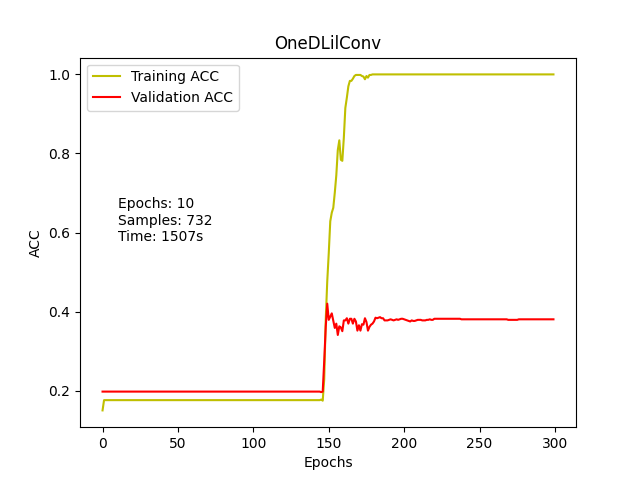
\includegraphics[height=5cm]{../../Plots/ba_plots/classnocascade/1dc.png}
    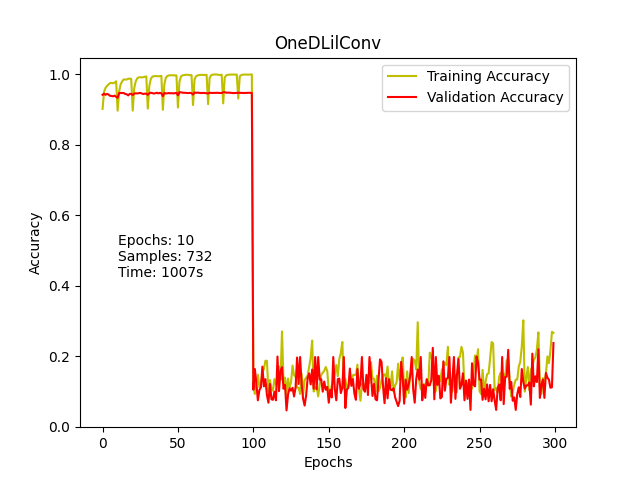
\includegraphics[height=5cm]{../../Plots/ba_plots/classTF/1dc_tr.png}
    \caption{\label{fig:timeother} 
    \small{In diesem Fall erfolgt das Training über eine hohe Anzahl an Epochen unter Einsatz tieferer und komplexerer Netzarchitekturen, 
    wodurch sich das Verhältnis der Trainingsdauer umkehrt. Veranschaulicht wird dies anhand der Tests 1DC:Comp/732//30 sowie 1DC:TF10/732/10/30.}}
\end{figure}

Wird mit einer höheren Anzahl an Epochen – beispielsweise 300 – und tieferen Netzarchitekturen trainiert, verschieben sich die zeitlichen 
Verhältnisse dahingehend, dass ein vollständig trainiertes Netzwerk mehr Zeit benötigt als ein kaskadiertes Transfer-Learning-Netzwerk. Diese 
Entwicklung ist in Abbildung \ref{fig:timeother} dargestellt.

Die Ursache hierfür liegt darin, dass ab einer bestimmten Netzwerktiefe und Epochenanzahl die Trainingsdauer nicht mehr primär durch 
strukturelle Aspekte – wie das Hinzufügen oder Entfernen von Layern oder die Berechnungszeit für den Augmented Vector – bestimmt wird, 
sondern maßgeblich vom eigentlichen Trainingsprozess.

Kaskadierte Netzwerke weisen in diesem Zusammenhang einen zeitlichen Vorteil auf, da sie jeweils nur die neu hinzugefügten Netzwerkbereiche 
trainieren müssen. Im Gegensatz dazu muss ein vollständiges Netzwerk sämtliche enthaltenen Layer kontinuierlich berücksichtigen, wobei diese 
während des Trainings einem fortlaufenden Änderungsprozess unterliegen. Dies führt zu häufigeren Gewichtsanpassungen und somit zu einem 
insgesamt höheren Rechenaufwand.
